\chapter{Revis{\~a}o da literatura correlata}\label{CAP_CORRELATOS}
\begin{flushright}
	\textit{``Não odeie seus inimigos. Isso afeta seu julgamento''(Vito Corleone)}
\end{flushright}

Este capítulo detalha os trabalhos presentes na literatura correlata analisados por meio de uma revisão sistemática. A seção \ref{SEC_METODOLOGIA_REVISAO} detalha as três fases da revisão sistemática: i) planejamento; ii) condução; e iii) extração de dados. A seção \ref{SEC_RESULTADOS_REVISAO} apresenta os artigos com técnicas correlatas na área de recomendação de atividades em \emph{workflows} científicos. A seção \ref{SEC_COMPARACAO_CORRELATOS} apresenta uma comparação entre a solução proposta, os trabalhos correlatos e com as restrições típicas de sistemas de recomendação de \emph{workflows} científicos (ver seção \ref{SEC_RECOMENDACAO_WORKFLOW_CIENTIFICO}).

\section{Metodologia da revisão sistemática} \label{SEC_METODOLOGIA_REVISAO}
A revisão iniciou com um estudo exploratório sobre o tema permitindo compreender o problema de recomendação em detalhes, encontrar termos específicos da área de \emph{workflows} científicos e definir palavras-chave. Em seguida, foi realizada uma revisão sistemática  composta por três etapas, como proposto por \citeonline{Biolchini2007}, sendo elas: i) planejamento; ii) condução; e iii) extração de dados. O objetivo dessa revisão foi responder à pergunta: ``Quais são as técnicas existentes para recomendar atividades em \emph{workflows}?''.

\subsection{Planejamento}
Nesta etapa, foram definidas: a pergunta que a revisão objetivou responder, as bibliotecas digitais utilizadas na pesquisa, a \emph{string} de busca e os critérios de inclusão e exclusão.

A revisão sistemática pretende responder a pergunta: ``Quais são as técnicas existentes para recomendar atividades em \emph{workflows}?''. Para responder a esta pergunta, foram selecionadas as bibliotecas digitais: ACMDL \cite{ACMDL}, IEEExplore \cite{IEEEXPLORE} e Science Direct \cite{ScienceDirect} por serem consideradas as principais bibliotecas digitais da área que disponibilizam artigos completos de diversos periódicos e conferências.

A \emph{string} de busca foi definida com auxílio da metodologia PICO \cite{Huang2006}, a qual define quatro grupos de palavras-chave e os relaciona com o operador \emph{AND}, os quais estão enumerados a seguir:
\begin{enumerate}
\item \textbf{Population:} \emph{scientific}, \emph{workflow} e \emph{pipeline};
\item \textbf{Intervention:} \emph{recommendation}, \emph{provenance}, \emph{suggestion}, \emph{forecast}, \emph{advice}, \emph{design}, \emph{visualization}, \emph{recommender}, \emph{construct}, \emph{proposal}, \emph{guidance}, \emph{counsel}, \emph{composition}, \emph{activity}, \emph{shimming}, \emph{inference}, \emph{reuse}, \emph{reusing}, \emph{semiautomatically}, \emph{similarity}, \emph{match}, \emph{matching}, \emph{complete}, \emph{auto};
\item \textbf{Control:} O alvo da pesquisa são as técnicas usadas;
\item \textbf{Output:} O alvo da pesquisa é descobrir como são validadas as técnicas propostas.
\end{enumerate}

Após definir os quatro grupos, foi especificada a seguinte \emph{string} de busca:
``(\emph{scientific} \textbf{and} (\emph{workflow} \textbf{or} \emph{pipeline})) \textbf{and} (\emph{recommendation} \textbf{or} \emph{provenance} \textbf{or} \emph{suggestion} \textbf{or} \emph{forecast} \textbf{or} \emph{advice} \textbf{or} \emph{design} \textbf{or} \emph{visualization} \textbf{or} \emph{recommender} \textbf{or} \emph{construct} \textbf{or} \emph{proposal} \textbf{or} \emph{guidance} \textbf{or} \emph{counsel} \textbf{or} \emph{composition} \textbf{or} \emph{activity} \textbf{or} \emph{shimming} \textbf{or} \emph{inference} \textbf{or} \emph{reuse} \textbf{or} \emph{reusing} \textbf{or} \emph{semiautomatically} \textbf{or} \emph{similarity} \textbf{or} \emph{match} \textbf{or} \emph{matching} \textbf{or} \emph{complete} \textbf{or} \emph{auto})''.

A \emph{string} de busca foi aplicada nas bases de dados selecionadas. Em seguida, foram lidos os resumos e conclusões de todos os artigos obtidos com a pesquisa e foram aplicados o critério de inclusão: i) artigos que utilizam técnica de recomendação de atividades em \emph{workflows}, e os de exclusão em todos os artigos: i) trabalhos não disponibilizados na integra; ii) trabalhos que não descrevem o método utilizado; e iii) trabalhos que não são da área de recomendação de atividades em \emph{workflows}. Para classificar um artigo como ``selecionado para leitura integral'', ele deve satisfazer o critério de inclusão e não satisfazer nenhum dos critérios de exclusão.

\subsection{Condução}
Submetendo-se a \emph{string} de busca nas bibliotecas digitais foram obtidos \(838\) artigos. Deste total, \(171\) oriundos da \emph{ACMDL}, \(448\) oriundos da \emph{IEEE} e \(219\) oriundos da \emph{Science Direct}. O resumo de cada artigo foi lido e os critérios de inclusão e exclusão aplicados. Após a aplicação deles, foram selecionados para a leitura integral \(24\) artigos, os quais estão exibidos em duas figuras: i) a figura \ref{fig:figArtigosPorBase}, que resume o resultado da aplicação dos critérios de inclusão e exclusão agrupados por base de dados; e ii) a figura \ref{fig:figArtigosPorAno}, que exibe a quantidade de artigos e o ano de sua publicação.
\begin{figure}[!hbt]
\centering
\caption{Artigos obtidos com a revisão sistemática}
\begin{subfigure}{.5\textwidth}
  \centering
  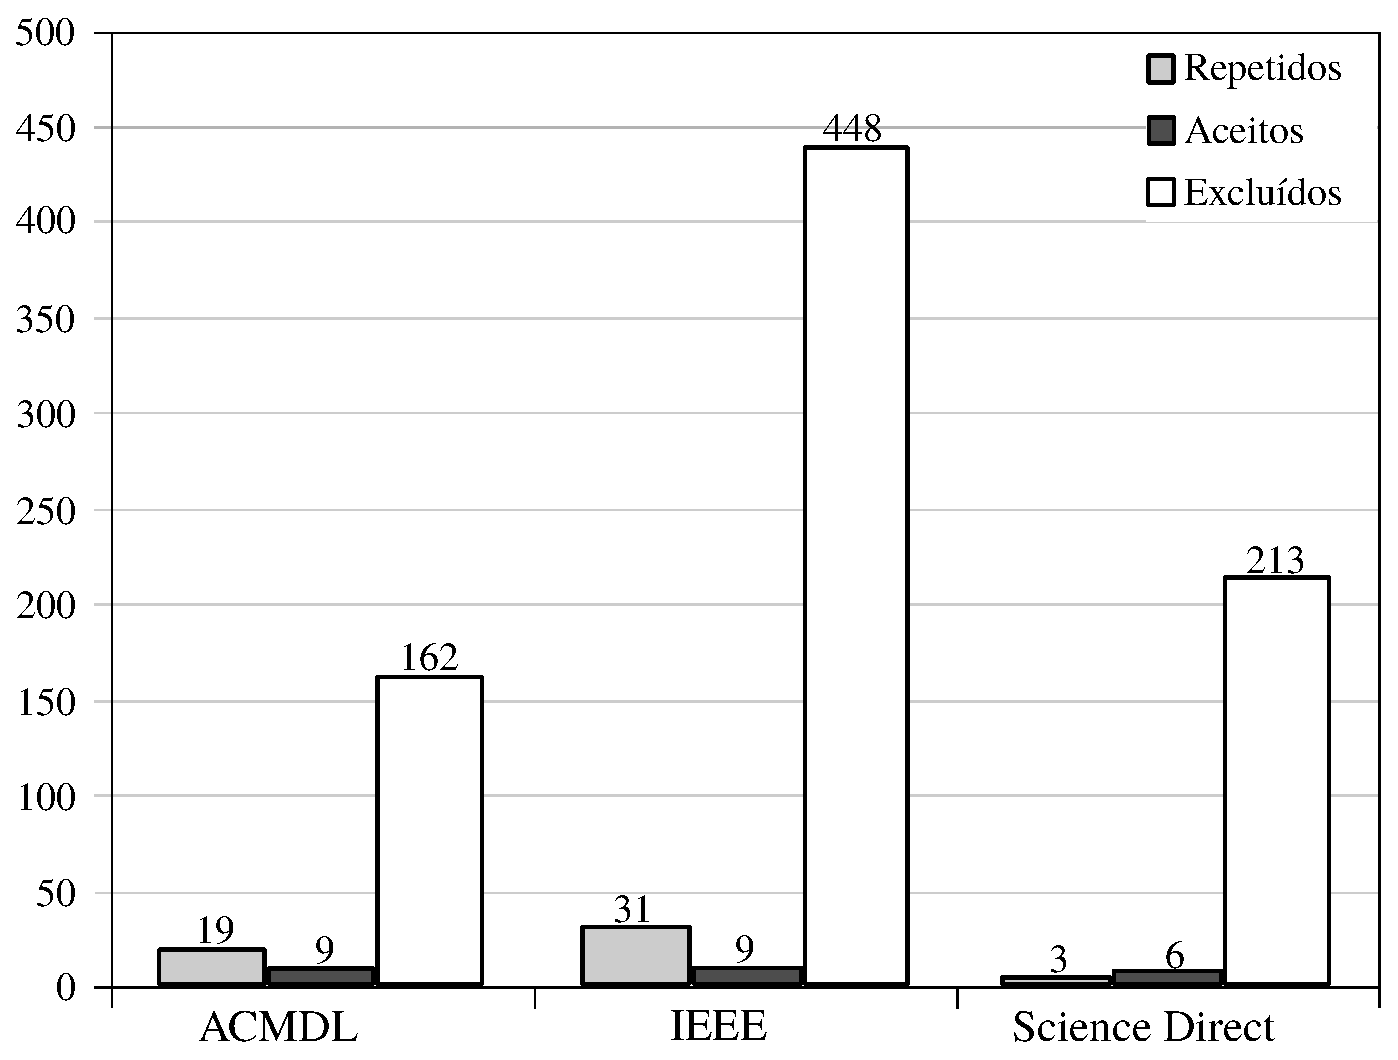
\includegraphics[width=7.5cm, height=5cm]{./secoes/correlatos/pics/img/GraficoQuantidade.eps}
  \caption{Agrupados por base de dados}
  \label{fig:figArtigosPorBase}
\end{subfigure}%
\begin{subfigure}{.5\textwidth}
  \centering
  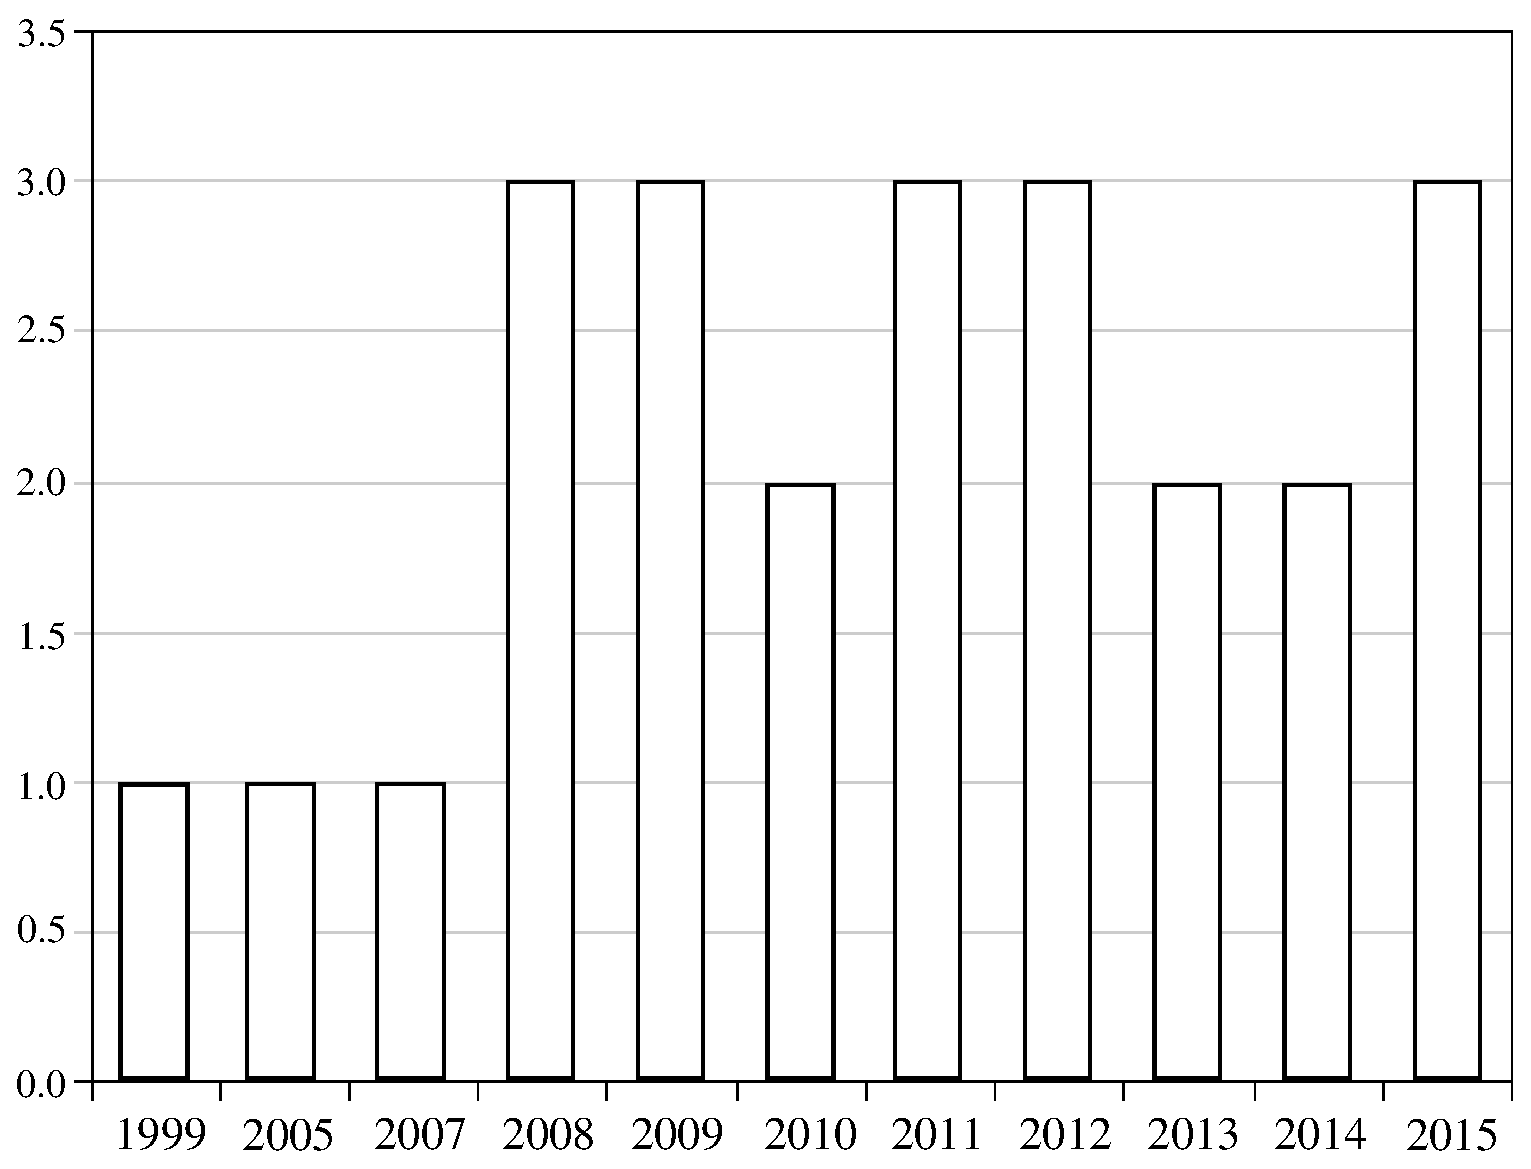
\includegraphics[width=7.5cm, height=5cm]{./secoes/correlatos/pics/img/GraficoQuantidadeAno.eps}
  \caption{Agrupados por ano de publicação}
  \label{fig:figArtigosPorAno}
\end{subfigure}
\label{fig}
\vspace{0.1cm}
 \source{\varAutorData}
\end{figure}

\subsection{Extração de dados}
Os dados extraídos de cada um dos artigos podem ser vistos na tabela \ref{tabResumoTecnicas}, junto com suas respectivas referências.

{\tiny
%	Abre ambiente para tabelas com mais de uma página.
\begin{longtabu} to \textwidth { |X[2.5,l]<{\strut}| X[2.0,l]<{\strut}| X[3.5,l]<{\strut}| }

%	Legenda e rótulo.
\caption{Técnicas da literatura correlata} \label{tabResumoTecnicas}
\\ \hline

%	Cabeçalho da primeira paǵina.
\multicolumn{1}{|c|}{\textbf{Referência}} & 
\multicolumn{1}{c|}{\textbf{Técnica}} & 
\multicolumn{1}{c|}{\textbf{Validação}} \\ \hline \endfirsthead

%	Cabeçalho repetido em todas as páginas.
\multicolumn{3}{c}
{ \tablename\ \thetable{} -- Continuação da página anterior} \\
\hline \multicolumn{1}{|c|}{\textbf{Referência}} &
\multicolumn{1}{c|}{\textbf{Técnica}} &
\multicolumn{1}{c|}{\textbf{Validação}}  \\ \hline
\endhead

%	Rodapé repetido em todas as páginas.
\hline \multicolumn{3}{|r|}{{Continua na próxima página}} \\ \hline
\endfoot
\endlastfoot
\cite{Telea1999}			& Frequência 							& Estudo de caso									\\ \hline

\cite{Bomfim2005}			& Ontologia 							& Estudo de caso									\\ \hline
	                 	
\cite{Shao2007}				& \emph{Itemsets} e proveniência de execução	& Estudo de caso									\\ \hline
                  	
\cite{Koop2008}				& Frequência e proveniências 			& \emph{Workflows} e suas proveniências				\\ \hline
                  	
\cite{Oliveira2008}			& Proveniências							& Estudo de caso									\\ \hline
                  	
\cite{Wang2008}				& Entrada e saída de atividades  		& Estudo de caso									\\ \hline
                  	
\cite{Shao2009}				& Proveniência de execução				& Estudo de caso									\\ \hline
                  	
\cite{Wang2009}				& \emph{Itemsets} e proveniência de execução	& Estudo de caso									\\ \hline
                  	
\cite{Zhang2009}			& Proveniência de modelagem				& Usados \emph{workflows} sintéticos 				\\ \hline 
                  	
\cite{Leng2010}				& Planejador							& Estudo de caso									\\ \hline 

\cite{Oliveir2010}			& Frequência							& Comparação com \citeonline{Koop2008}				\\ \hline 
                 	
\cite{Cerezo2011}	  		& Entrada/saída e semântica				& Estudo de caso									\\ \hline
                 	
\cite{Tan2011}				& Proveniência de execução				& Estudo de caso									\\ \hline 
                 	
\cite{Zhang2011}			& Frequência							& Dados do \emph{myExperiment} \cite{ROURE2015}		\\ \hline 
                 	
\cite{Cao2012}				& Proveniência de modelagem				& Comparado com \citeonline{Zhang2009}				\\ \hline 
                 	
\cite{Diamantini2012}		& Proveniência de modelagem				& Dados do \emph{myExperiment} \cite{ROURE2015}		\\ \hline 
                 	
\cite{Yao2012}				& Baseado em confiança					& Dados do \emph{myExperiment} \cite{ROURE2015}		\\ \hline
                 	
\cite{Garijo2013}			& Frequência e proveniência de execução	& Dados do SGWC \emph{Wings} \cite{Wings2015} 		\\ \hline 
                 	
\cite{Yeo2013}				& Proveniência de execução				& Dados do \emph{myExperiment} \cite{ROURE2015}		\\ \hline 
		
\cite{Zhang2014}			& Frequência e anotações			 	& Interfaces do \cite{ProgrammableWeb}				\\ \hline 

\cite{CorchoGarijo2014} 	& Frequência e Ontologia			  	& Dados da plataforma LONI \cite{Rex2003}			\\ \hline

\cite{TostaBraganholo2015}	& \emph{Itemsets} considerando ordem	& Comparação com \citeonline{Koop2008}				\\ \hline

\cite{Mohan2015}			&  Entrada/saída e semântica			& Dados do \emph{myExperiment} \cite{ROURE2015}		\\ \hline

\cite{Soomro2015}			& Frequência e Ontologia				& Dados da plataforma LONI \cite{Rex2003}			\\ \hline
\caption*{{\footnotesize Fonte: \varAutorData } }
\end{longtabu}
%\source{\varAutorData}
%\source{\varAutorData}
}

\section{Análise dos artigos selecionados pela revisão sistemática}\label{SEC_RESULTADOS_REVISAO}
Nesta seção são apresentadas as técnicas para recomendar atividades em \emph{workflows} científicos, empregadas ou propostas pelos trabalhos retornados pela revisão da seção \ref{SEC_METODOLOGIA_REVISAO}.

O sistema \emph{Smartlink}, proposto por \citeonline{Telea1999}, modela os \emph{workflows} científicos como grafos, nos quais as arestas correspondem ao fluxo de dados e os nós às atividades. É criado um grafo das atividades mais utilizadas e elaborada uma busca em profundidade procurando por atividades. A recomendação do \emph{Smartlink} é baseada no grafo de atividades mais utilizadas, o que permite minimizar os seguintes problemas: i) Como conectar duas atividades?; e ii) Quais atividades podem ser conectadas a uma atividade específica? A estratégia de recomendação não foi testada e comparada com a literatura, foi apenas implementada em alguns sistemas e usada.

\citeonline{Bomfim2005} desenvolveram um sistema de recomendação de atividades em \emph{workflows} científicos baseado em ontologia de domínio que é utilizada para recomendar atividades em \emph{workflows}. São comparadas as anotações da proveniência de modelagem com as do \emph{workflow} em construção e são recomendados os \emph{workflows} que contenham os mesmos conceitos ontológicos. A proposta não considera as dependências de dados e de controle para recomendar atividades. Além disso, a qualidade da recomendação não foi testada e os autores não detalharam a ontologia construída.

\citeonline{Shao2007} e \citeonline{Shao2009} propõem minerar a proveniência de execução para encontrar os experimentos que terminam em estado de sucesso. As execuções dos \emph{workflows} são modeladas como grafos acíclicos dirigidos. Cada execução parte do estado inicial até atingir um dos estados finais: i) teste; ii) não finalizado; iii) irrelevante, que não auxilia a atingir o estado de sucesso; e iv) sucesso. São considerados críticos todos os caminhos que partem do estado inicial e terminam no estado sucesso. Não foram realizados experimentos sobre recomendação, apenas sobre tempo de execução para minerar a proveniência. Os autores citam que essas técnicas poderiam ser utilizadas para recomendar os \emph{subworkflows} de sucesso para os \emph{workflows} em construção.

\citeonline{Koop2008} recomenda \emph{subworkflows} frequentes considerando a estrutura do \emph{workflow}. Para tal, são encontradas (utilizando a proveniência de execução) todas as sequências de atividades posteriores ao nó âncora (aquele que vem antes do item a ser recomendado). Essas atividades serão recomendadas ao usuário. Os testes utilizaram \(2.875\) \emph{workflows} e suas proveniências de execução, geradas por estudantes durante um curso de visualização de dados. O conjunto de dados foi dividido em: i) treinamento, responsável por gerar caminhos; e ii) testes, responsável por usar caminhos gerados e recomendar.

\citeonline{Oliveira2008} propõem recomendar trechos de \emph{workflows} baseado em filtro colaborativo sobre a proveniência de execução e de modelagem de outros \emph{workflows}. Sempre que uma atividade é adicionada, o sistema verifica quais as atividades seguintes foram utilizadas, considerando os dados de proveniência, e recomendando-as. Esta estratégia não foi comparada com a literatura, foi apenas implementada no SGWC Vistrails \cite{Vistrails} e foi apresentada uma recomendação de uma atividade.

Na área de recomendação de serviços, \citeonline{Wang2008} recomendam serviços baseados nos fatores dependência entre serviços, modelos existentes e ordem de execução dos serviços. Considere um modelo de \emph{workflow} no qual um serviço ``b'' invoca um serviço ``c'' e o serviço ``c'' invoca o serviço ``d''. Em um \emph{workflow} em construção, após a inclusão do nó ``b'', serão dadas as recomendações ``c'' e ``d'' ordenadas pela proximidade com ``b''. A técnica foi testada em dois problemas da área de bioinformática, porém não ocorreu uma comparação com a literatura correlata.

\citeonline{Zhang2009} propõem uma estratégia de recomendação baseada no subgrafo anterior ao nó âncora (aquele que vem antes do item a ser recomendado) que é definido por meio da proveniência de modelagem. São recomendados os nós posteriores aos subgrafos com maior ocorrência, isto é, é gerada uma lista com todas as possibilidades de próximos nós baseados em todos os nós anteriores ao nó âncora, de acordo com a proveniência de modelagem. Esta estratégia foi testada por meio de \emph{workflows} e proveniências criados pelos autores.

\citeonline{Wang2009} recomendam atividades por meio de \emph{itemsets} frequentes minerados a partir das mudanças ocorridas nos \emph{workflows}. Cada mudança é denominada \(\Delta\), uma série destas transforma um \emph{workflow} em outro e consiste na sequência: \(\Delta_{0}, \Delta_{1}, \ldots, \Delta_{N}\). É aplicado o algoritmo \emph{Apriori} em todas as sequências de operações \(\Delta\). Dessa forma, são obtidas as regras de associação que podem ser usadas como recomendação. A técnica é implementada em um SGWC, porém não ocorrem comparações com a literatura correlata.

\citeonline{Leng2010} propõem um planejador que procura por termos de uma ontologia. Primeiramente, os grafos acíclicos dirigidos, que representam os serviços web e suas relações, são modelados como uma quíntupla (P, \(P_{0}\), G, A, \(\Gamma\)) onde P é o conjunto de proposições, \(P_{0}\) é o estado inicial, G é o estado a ser atingido, A é o conjunto de ações que transformam uma proposição em outra e \(\Gamma\) é a função que transforma proposições. 

No grafo, os serviços serão as ações A, as entradas e saídas de todos os serviços serão as proposições P, a entrada passada pelo usuário será o estado inicial \(P_{0}\) e a saída esperada pelo usuário será o estado final a ser atingido G. O planejador começa adicionando os estados que satisfaçam as entradas das proposições existentes e que tenham uma similaridade semântica mínima, a qual é calculada por meio de graus de similaridade comparando as anotações semânticas feitas em todos os serviços com termos controlados por uma  ontologia. 

A similaridade entre dois conceitos, \(c_{1}\) e \(c_{2}\), da ontologia é calculada com as seguintes regras: i) \(c_{1}\) e \(c_{2}\) são equivalentes, então é denominada exata; ii) \(c_{2}\) é super conceito de \(c_{1}\); iii) \(c_{1}\) é super conceito de \(c_{2}\); iv) são inexatos. Ao término do algoritmo é encontrado um caminho entre o estado inicial e o final o qual é recomendado. O sistema foi parcialmente testado, pois ainda estava sendo implementado, porém não ocorreram comparações com a literatura correlata, apenas uma recomendação específica para um caso simples.

\citeonline{Oliveir2010} recomenda atividades de \emph{workflows} científicos utilizando mineração sequencial. Essa abordagem permite utilizar uma modificação do algoritmo \emph{Preorder Linked WAP} (PLWAP) desenvolvido por \citeonline{Ezeife2005} para recomendar atividades. São determinadas as sequências maximais (aquelas que não estão presentes em outras sequências de um mesmo \emph{workflow}). As sequências são a entrada para o PLWAP que define os caminhos padrões (que são usados como recomendação). Foi usada uma base de dados de \(3.340\) \emph{workflows}, essa estratégia de recomendação foi comparada com a proposta por \citeonline{Koop2008}.

\citeonline{Cerezo2011} elaboraram um sistema que permite construir \emph{workflows} em alto nível, utilizando ontologias de domínio. Essa modelagem é convertida para uma linguagem que pode ser executada por sistemas gerenciadores de \emph{workflow} científico. Durante a tradução, que é semiautomática, são recomendados para o usuário \emph{subworkflows} que possuem entradas e saídas compatíveis sintaticamente e cuja similaridade ontológica é alta em relação ao \emph{workflow} de alto nível modelado. Os autores não citam a estratégia de validação dos resultados, apenas elaboram uma recomendação específica para um caso simples.

\citeonline{Tan2011} constroem dois grafos: i) \emph{workflows} e seus serviços, representados por nós, e as arestas representam a relação de inclusão de um serviço dentro de um \emph{workflow}; e ii) entre operações, em que os nós representam operações dentro de serviços e as arestas operações entre serviços. Com esses grafos, é possível usar o algoritmo \emph{Apriori} para descobrir quais serviços são utilizados em conjunto por quais usuários, e assim gerar recomendações. Não são citadas comparações com a literatura correlata, apenas uma recomendação específica para um caso simples.

\citeonline{Zhang2011} constroem redes sociais de: i) \emph{workflows} e serviços; ii) serviços e serviços; e iii) pessoas e serviços. As redes permitem avaliar quais serviços são utilizados por quais \emph{workflows}, com qual frequência e quem são os autores. O sistema foi testado com \emph{workflows} do repositórios \emph{myExperiment} \cite{ROURE2015} com validação cruzada, são recomendados os serviços mais frequentemente utilizados em \emph{workflows} distintos.

No contexto de processos de negócio, \citeonline{Cao2012} aplicam recomendação baseada em grafos durante a construção dos \emph{workflows}. Os grafos prontos são minerados para definir padrões (sequências frequentes). Em seguida, é calculada a distância entre os padrões e o processo de negócio (\emph{workflow}) em construção. Os padrões com menor distância em relação ao processo de negócio em construção são recomendados ao usuário. A distância é calculada utilizando uma métrica elaborada pelos autores que considera a posição do nó no modelo pronto e no subgrafo em construção. A técnica foi comparada com a proposta de \citeonline{Zhang2009}.

\citeonline{Diamantini2012} recomendam fragmentos de \emph{workflows}, modelados como um grafo dirigido acíclico, encontrando as menores subestruturas mais representativas de cada grafo. Para tal, empregam um algoritmo de agrupamento da biblioteca SUBDUE que permite reduzir os nós do grafo utilizando a métrica \emph{Minimum Description Length} (MDL)
\begin{align}
MDL = \frac{DL(S)+DL(G|S)}{DL(G)} \label{EQU_MDL}
\end{align}
em que \(DL(S)\) é a \emph{Description Length} (DL), que é uma função para computar o número de \emph{bits} necessários para representar a matriz de adjacência do subgrafo \(S\), \(DL(G)\) é a \emph{Description Length} do grafo original \(G\) e \(DL(G|S)\) \emph{Description Length} de \(G\) comprimido por \(S\). São recomendados os padrões mais representativos ordenados pelo valor da equação \eqref{EQU_MDL}. Para teste foi utilizado um subconjunto de \(564\) \emph{workflows} do repositório \emph{myExperiment} \cite{ROURE2015} obtendo como saída uma hierarquia de agrupamentos similares que, segundo os autores, poderiam ser usados para a recomendação.

\citeonline{Yao2012} recomendam com base na confiabilidade de serviços e autores: a \emph{ReputationNet} que é um sistema de recomendação de atividades para \emph{workflows} que considera a reputação do autor (escolaridade, especialidade e número de citações) e a popularidade dos serviços (frequência relativa). Os serviços mais populares dos autores mais confiáveis são recomendados. Foram utilizados diversos \emph{workflows} do repositório \emph{myExperiment} \cite{ROURE2015} para validar os resultados.

\citeonline{Garijo2013} mineram a proveniência de execução para encontrar fragmentos frequentes de \emph{workflows} e recomendá-los. Os rastros de proveniência são representados como grafos dirigidos acíclicos. Dado um repositório de \emph{workflows} e sua proveniência de execução, o objetivo é encontrar: i) conjuntos de atividades frequentes; e ii) \emph{subworkflows} frequentes, utilizando o algoritmo de agrupamento do SUBDUE (baseado na equação MDL). Os testes foram feitos com \(22\) \emph{workflows} e suas proveniências. O resultado de estruturas frequentes encontradas foi comparado com os resultados de uma pesquisa manual. A diferença entre esta proposta e a de \citeonline{Diamantini2012} é que esta considera a proveniência de execução para recomendar, a outra apenas os \emph{workflows} prontos.

\citeonline{Yeo2013} adaptam a técnica de rastro de causalidade para \emph{workflows} científicos, originalmente esta técnica foi usada em \emph{workflows} de negócios. Para isto, os autores armazenam a informação de fluxo dos dados junto com o grafo de causalidade para \emph{workflows} científicos 
\begin{align}
G = <N, DP, L_{B}, L_{A}>
\end{align}
em que \(N\) é o número de atividades, \(DP\) é o conjunto de caminhos do fluxo de dados, \((A, b) \in L_{B}\) é o conjunto de atividades anteriores, tal que a execução de \(b\) é sempre realizada após alguma atividade do conjunto \(A\) e \((a, B) \in L_{A}\) é o conjunto de nós posteriores, tal que \(a\) é sempre executada antes de alguma das atividades do conjunto \(B\).

Utilizando o rastro é possível criar um vetor de distâncias entre o nó âncora (que será alvo da recomendação) e os possíveis próximos nós, oriundos de \(L_{A}\). Esse vetor booleano contém o valor \emph{um} representando a presença de uma atividade do rastro e \emph{zero} caso contrário. Os vetores são gerados para todos os rastros da base de dados e suas similaridades são calculadas por meio da similaridade do cosseno \cite{Deza2009}. Foram usados \(12\) \emph{workflows} do repositório \emph{myExperiment} \cite{ROURE2015} modificados para receber a recomendação. A modificação consistia na remoção de uma atividade enquanto se esperava que o sistema a recomendasse.

\citeonline{Zhang2014} constroem uma rede social de \emph{workflows} e serviços (os quais são os nós) e suas possíveis relações (que são as arestas) são do tipo de inclusão ou de autoria. Essa rede pode ser modelada como uma matriz \(Q\) em que \(q_{i, j} = 1\) indica a inclusão do serviço \emph{i} no \emph{workflow} \emph{j} ou como a matriz \(S = Q^{T}Q\) em que \(s_{i, j}\) representa o número de \emph{workflows} nos quais os serviços (\(i, j\)) são chamados. 

Quanto mais vezes dois serviços são utilizados em \emph{workflows}, maior o grau de ligação entre os mesmos. Todos os serviços são publicados com metadados. Dessa forma, os autores calculam o \emph{Term Frequency-Inverse Category Frequency} (TF-ICF) nos metadados que descrevem os serviços e suas categorias. Com base nos valores de TF-ICF cada serviço é classificado em \(k\) categorias. Durante a construção do \emph{workflow} são sugeridos serviços de acordo com a métrica \emph{Rank-Biased Overlap} (RBO), descrita no artigo. São recomendados os serviços que possuem maior RBO em relação ao \emph{workflow} em construção. São usados serviços da plataforma \citeonline{ProgrammableWeb} para validar os resultados.

\citeonline{CorchoGarijo2014} recomendam atividades baseados em algoritmos de mineração de grafos para encontrar os \emph{subworkflows} mais frequentes e recomendá-los. A similaridade entre eles e o \emph{workflow} em construção é dada pela métrica MDL (ver equação \ref{EQU_MDL}). Como parâmetros, o usuário deve estabelecer o tamanho mínimo e máximo dos \emph{subworkflow} a serem recomendados. O algoritmo modela o problema como um grafo dirigido, em seguida calcula os fragmentos mais frequentes. Por fim, usa uma ontologia que relaciona os \emph{subworkflows} com os \emph{workflows}. Para validar a proposta, o sistema foi usado por usuários que compararam os \emph{subworkflows} gerados e sugeridos com \emph{subworkflows} que eles procuraram manualmente.

\citeonline{TostaBraganholo2015} recomendam atividades baseados em algoritmos de mineração sequencial (como \citeonline{Agrawal1994}), adaptados para considerar a ordem das atividades. A técnica pesquisa os \emph{itemsets} com confiança e suporte mínimos estabelecidos e recomenda-os durante a construção do \emph{workflow} científico considerando a ordem das atividades. Essa técnica foi comparada com o trabalho de \citeonline{Koop2008} (em termos de consumo de memória e tempo gasto para gerar subgrafos) para sua validação.
 
\citeonline{Mohan2015} desenvolveram uma plataforma \emph{web}, com a funcionalidade de recomendar \emph{workflows} finalizados da base de dados, a qual permite construir \emph{workflows} e anotá-los semanticamente usando \emph{tags} criadas pelo usuário. Durante a construção do \emph{workflow} o sistema pesquisa por todos os \emph{workflows} da base que contenham entrada compatível com a saída do \emph{workflow} em construção e analisa quais contêm as mesmas anotações semânticas que as do perfil do usuário e os recomenda. A validação ocorreu usando \(9.886\) usuários, \(2.664\) \emph{workflows} e \(9.624\) \emph{tags} do repositório \emph{myExperiment} \cite{ROURE2015}.

\citeonline{Soomro2015} criaram um sistema de recomendação baseado em mapeamento de atividades em conceitos ontológicos funcionais acrescido de semântica de dados oriunda de uma ontologia de domínio. Durante a construção do \emph{workflow}, cada uma de suas atividades é mapeada em um conceito ontológico, em seguida a base de dados recomenda todos os \emph{subworkflows} que contenham aqueles conceitos ontológicos naquela sequência ordenados pela sua frequência. Os testes foram realizados com \(65\) \emph{workflows} da plataforma LONI \cite{Rex2003} usando a métrica MRR. Os autores não citam detalhes da ontologia usada.

\section{Tendências observadas com os resultados da revisão sistemática}
A partir da figura \ref{figTecnicasPorQuantidade} é possível notar a existência de uma tendência no uso de técnicas baseadas em proveniência de dados, frequência e dependência da informação. A partir de \(2014\) a literatura começou a considerar estratégias híbridas que usam proveniência e algum tipo de informação semântica. No ano de \(2015\) foram publicados dois artigos propondo estratégias híbridas para recomendar que usam frequência e algum tipo de informação semântica para recomendar \emph{subworkflows}.
\begin{figure}[H]
	\centering
 	  \caption{Número de artigos por técnica de recomendação}
		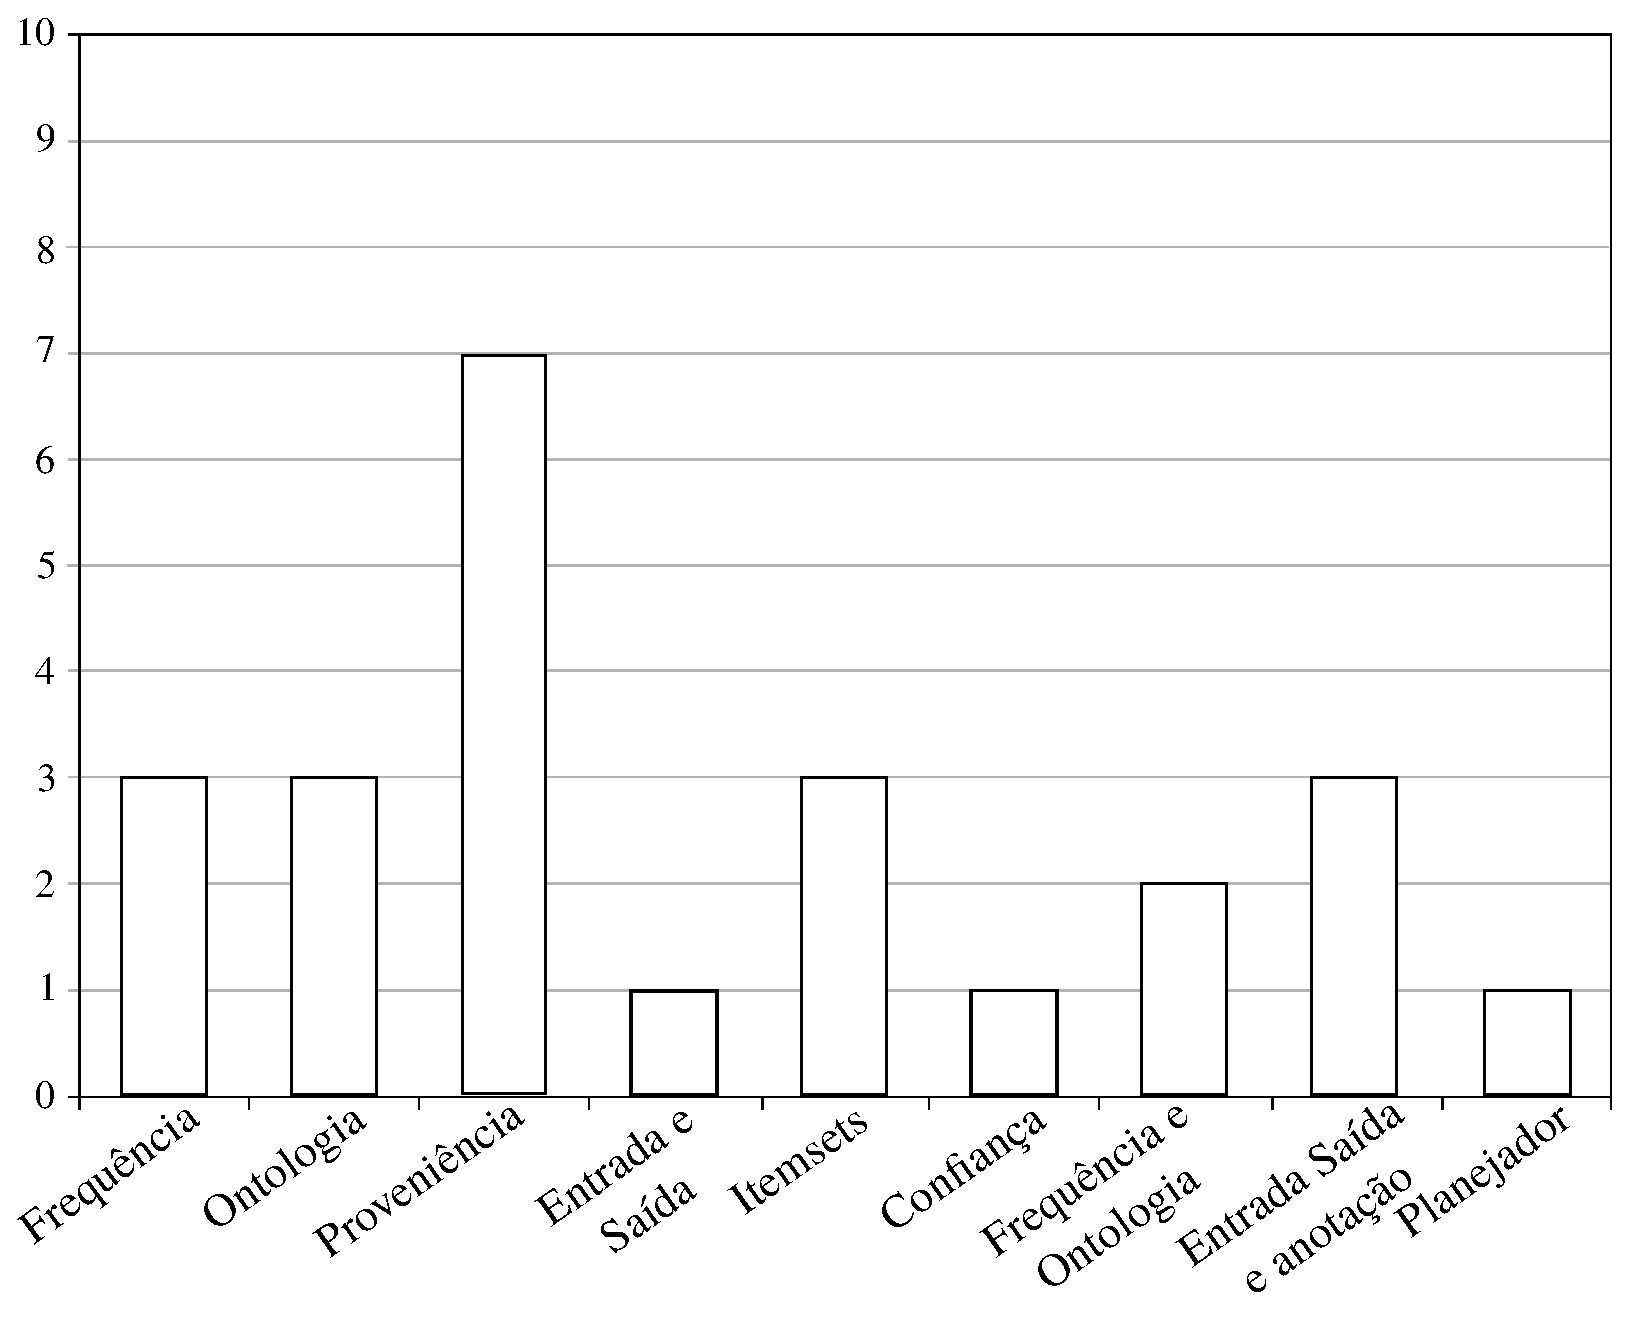
\includegraphics[width=11cm,height=6cm]{./secoes/correlatos/pics/img/GraficoQuantidadeTecnica.eps}
	\label{figTecnicasPorQuantidade}
  	\source{\varAutorData}
\end{figure}

A técnica baseada em proveniência de dados (mais utilizada na literatura) tem como vantagem considerar diversos dados históricos sobre um mesmo padrão de atividade. Por exemplo, para recomendar uma atividade em um \emph{workflow} que contenha a atividade~x, são considerados todos os \emph{workflows} que contenham x e suas atividades posteriores, a atividade com maior frequência é recomendada. Essa abordagem permite minimizar o efeito de \emph{outliers}. Como desvantagem, possui a necessidade de uma base de dados históricos relevantes, caso contrário, \emph{outliers} podem afetar o desempenho.

A técnica baseada em frequência tem como vantagem a simplicidade na implementação e como principal desvantagem a necessidade de uma base de dados com pouca esparsidade no uso de atividades.

A técnica baseada em dependência de informação tem como principal vantagem a facilidade de implementação. Como desvantagem, ela não leva em consideração a semântica dos dados das atividades. Por exemplo, uma \emph{string} que representa o nome de uma espécie de bactéria é considerada similar a uma \emph{string} que representa um CEP.

Outra tendência observada é sobre a validação dos resultados. Não há uma metodologia amplamente utilizada entre os trabalhos analisados para validação. Muitos autores apenas executam a solução uma vez para ``mostrar'' que sua solução funciona. Não ocorrem testes com dados sintéticos ou reais, o que pode ser verificado na tabela \ref{tabResumoTecnicas} em que \(11\) artigos estão nessa situação (marcados na tabela como ``Elaborado um estudo de caso'').

\section{Comparação da solução proposta com os trabalhos correlatos}\label{SEC_COMPARACAO_CORRELATOS}
Nesta seção são comparadas as técnicas descritas com o projeto deste mestrado em relação as restrições típicas de sistemas de recomendação de \emph{workflows} científicos, que foram detalhadas na seção \ref{SEC_RECOMENDACAO_WORKFLOW_CIENTIFICO} do capítulo de conceitos fundamentais.

Os trabalhos de \citeonline{Shao2007} e \citeonline{Shao2009}, que consideram a mineração sequencial de atividades como \emph{itemsets} desconsideram a ordem das atividades e a semântica das mesmas. A proposta de \citeonline{TostaBraganholo2015} desconsidera apenas a semântica das atividades. Esta proposta de mestrado considera a ordem de atividades que é um fator importante na recomendação conforme visto no capítulo de conceitos fundamentais.

Os trabalhos de \citeonline{Koop2008, Oliveira2008, Wang2009, Zhang2009, Tan2011, Cao2012, Diamantini2012, Garijo2013, Yeo2013} consideram a ordem das atividades, entrada e saída e proveniência dos dados. Suas limitações são a necessidade de dados de proveniência, pois nem todo SGWC armazena essas informações, além de desconsiderar informação semântica dos \emph{workflows} e atividades. Este projeto não necessita de informações de proveniência e considera a semântica da informação por meio de uma ontologia hierarquizada e validada por um especialista da área.

O trabalho de \citeonline{Bomfim2005} usa apenas um mapeamento entre atividades e ontologia desconsiderando a entrada e saída, o que potencialmente gera recomendações ineficientes. Neste projeto são consideradas às entradas e saídas de cada atividade individualmente, além do uso de uma ontologia de domínio.

\citeonline{Wang2008, Leng2010} desconsideram o uso de semântica das atividades e da frequência de suas ocorrências em pares. Nesse projeto de mestrado são considerados esses dois fatores.

O trabalho de \citeonline{Yao2012} exige dados que permitam calcular a confiança dos usuários e dos seus \emph{workflows}. Repositórios como \emph{myExperiment} \cite{ROURE2015} não exigem dos usuários o preenchimento de todos os seus dados, de forma que grande parte das informações relacionadas a este aspecto não são preenchidas pelos usuários. Além disso, os autores desconsideram a semântica das atividades e \emph{workflows}. Este projeto de mestrado considera a semântica de \emph{workflows} e não necessita da informação sobre a confiança dos usuários.

Os trabalhos de \citeonline{Telea1999, Oliveir2010} e \citeonline{Zhang2011} desconsideram o uso de semântica de dados para recomendar, o que é um limitante conforme discutido por \citeonline{CorchoGarijo2014, Soomro2015}. No presente mestrado, a frequência é considerada em conjunto com a ontologia de domínio.

Os trabalhos de \citeonline{Zhang2014, Mohan2015, Cerezo2011} desconsideram o uso de uma ontologia hierarquizada e validada por um especialista. Dessa forma, a qualidade das anotações semânticas é questionável. Nesse projeto foi construída uma ontologia usando uma metodologia e esta foi validada por um especialista.

Os trabalhos de \citeonline{CorchoGarijo2014, Soomro2015} consideram o uso de frequência e ontologia, como neste projeto, porém recomendam \emph{subworkflows} o que limita as recomendações de atividades. Apenas atividades usadas em fragmentos comuns de \emph{workflows} poderão ser recomendadas. Em outras palavras, se a atividade se encontra no ``meio'' de um \emph{subworkflow} esta nunca poderá ser recomendada individualmente. No presente mestrado, todas as atividades tem possibilidade de ser recomendadas, mesmo que no final da lista de recomendação. Além disso, apresenta uma recomendação mais abrangente, pois trata o caso de atividades simples, \emph{subworkflows} e \emph{Shims} (ver seção \ref{SEC_CONSTRUCAO_WORKFLOWS_CIENTIFICOS}).

Neste mestrado o problema de recomendação de atividades foi também modelado como um problema de classificação e regressão, usando para isso \(5\) classificadores; \(5\) regressores; um classificador SVM composto (que usa o resultado dos outros classificadores e regressores para recomendar) e um \emph{ensemble} de classificadores (\emph{Rotation Forest}).
